\documentclass[11pt,a4paper]{article}
\usepackage[utf8]{inputenc}
\usepackage{amsmath,amssymb,amsfonts}
\usepackage{geometry}
\usepackage{graphicx}
\usepackage{booktabs}
\usepackage{hyperref}
\usepackage{bm}
\usepackage{tikz}
\usetikzlibrary{calc, patterns, angles, quotes}

\geometry{top=2.5cm, bottom=2.5cm, left=2.5cm, right=2.5cm}

\title{\textbf{Modellazione Dinamica di un Sistema Carrello-Multi-Link con Carico Rettangolare via Eulero-Lagrange}}
\author{\textbf{Alessandro Prisco} \\ Università degli Studi di Napoli Federico II}
\date{\today}

\begin{document}
	
\section*{4. PROPOSED CONTROL METHOD}

\subsection*{4.1 Definition of output function}

In this section we will consider a control method for the three link acrobat robot instead of for the two link robot. For the control problem of the three link robot there exist two basic approaches. One is that first dynamics is reduced into that of two link system using a variable constraint control$^{7)}$ or a dead beat controller$^{8)}$, and the control method in the previous section is applied for. The control method,however, may require conservative control input and it is difficult to analyze the performance based on a linear model. The other one is that a new output function is defined to the problem, and a zeroing controller is constructed. In this paper we adopt the latter approach.

In a paper by$^{4)}$ it was pointed out in theory that there should exist two output functions with which output zeroing stabilizes the three link robot, however, such functions have not been found analytically. Since the angular momentum of the three link robot is not integrable, we can not define a proper output function from the momentum analytically. So we propose a method in which integrable function is approximated based on the angular momentum then the integral function is determined. In the actual algorithm they are done simultaneously.
	\subsection*{4.2 Modeling of three link robot}
	
	We consider a three link robot shown in Fig.3 where $\theta_1, \theta_2, \theta_3$ are measured from the vertical axis.
	
	\begin{center}
		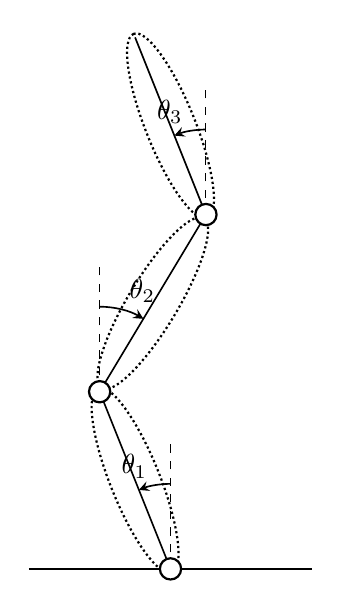
\begin{tikzpicture}[scale=0.9]
			% Definizione delle coordinate dei giunti
			\coordinate (O)  at (0,0);
			\coordinate (P1) at (-1, 2.5);
			\coordinate (P2) at (0.5, 5);
			\coordinate (P3) at (-0.5, 7.5);
			
			% Linea di terra (Ground)
			\draw[thick] (-2, 0) -- (2, 0);
			
			% Linee verticali tratteggiate di riferimento
			\draw[dashed] (O) -- (0, 1.8);
			\draw[dashed] (P1) -- ($(P1) + (0, 1.8)$);
			\draw[dashed] (P2) -- ($(P2) + (0, 1.8)$);
			
			% Sagome dei link (ellissi puntinate)
			% Link 1: inclinazione 111.8 gradi, centro a (-0.5, 1.25)
			\draw[densely dotted, thick, rotate around={111.8:(-0.5, 1.25)}] (-0.5, 1.25) ellipse (1.4 and 0.35);
			% Link 2: inclinazione 59.0 gradi, centro a (-0.25, 3.75)
			\draw[densely dotted, thick, rotate around={59:(-0.25, 3.75)}] (-0.25, 3.75) ellipse (1.4 and 0.35);
			% Link 3: inclinazione 111.8 gradi, centro a (0, 6.25)
			\draw[densely dotted, thick, rotate around={111.8:(0, 6.25)}] (0, 6.25) ellipse (1.4 and 0.35);
			
			% Scheletro interno dei link
			\draw[semithick] (O) -- (P1) -- (P2) -- (P3);
			
			% Archi per gli angoli theta
			\draw[->, >=stealth, semithick] (0, 1.2) arc[start angle=90, end angle=111.8, radius=1.2] node[midway, above left=-1pt] {$\theta_1$};
			\draw[->, >=stealth, semithick] ($(P1)+(0, 1.2)$) arc[start angle=90, end angle=59, radius=1.2] node[midway, above right=-1pt] {$\theta_2$};
			\draw[->, >=stealth, semithick] ($(P2)+(0, 1.2)$) arc[start angle=90, end angle=111.8, radius=1.2] node[midway, above left=-1pt] {$\theta_3$};
			
			% Disegno dei giunti (cerchi bianchi con bordo)
			\filldraw[fill=white, thick] (O) circle (0.15);
			\filldraw[fill=white, thick] (P1) circle (0.15);
			\filldraw[fill=white, thick] (P2) circle (0.15);
		\end{tikzpicture}
		
		\vspace{0.3cm}
		Fig. 3: Three link acrobat robot.
	\end{center}
	
	\vspace{0.2cm}
	The control purpose is to drive the state to upright position, i.e.
	$$ \bm{\theta} := [ \ \theta_1 \quad \theta_2 \quad \theta_3 \ ] \rightarrow [ \ 0 \quad 0 \quad 0 \ ] . $$
	
	The inertia matrix of the system can be represented as
	$$ \bm{M}(\bm{\theta}) = 
	\begin{bmatrix}
		a_{11} & a_{12}\cos(\theta_2 - \theta_1) & a_{13}\cos(\theta_3 - \theta_1) \\
		a_{12}\cos(\theta_2 - \theta_1) & a_{22} & a_{23}\cos(\theta_3 - \theta_2) \\
		a_{13}\cos(\theta_3 - \theta_1) & a_{23}\cos(\theta_3 - \theta_2) & a_{33}
	\end{bmatrix}
	$$
	where $a_{11}, a_{12}, a_{13}, a_{22}, a_{23}, a_{33}$ are constant coefficients depending on the physical parameters.
	\subsection*{4.3 Output function and zeroing controller}
	
	For the three link acrobat robot, $L$ is not integrable, however, an approximated function of $L$ may be integrable. If such a function is found, zero dynamics can be stabilized using the angular momentum.
	
	In order to approximate the function $\hat{p}$, we employ Radial Basis Function (RBF) Neural network due to simplicity of the construction and of the implementation to a real time control. For the radial basis function Gaussian type basis function is used. Please notice here that we restrict that $\phi$ is a function of only $\theta$ and $\hat{p}$ is defined as
	\begin{equation}
		\hat{p} = \sum_{i}^{n} w_i \phi_i(\theta_1, \theta_2, \theta_3), \tag{21}
	\end{equation}
	
	\begin{equation}
		\phi_i(\theta_1, \theta_2, \theta_3) = \exp \left( \frac{-\| \theta - \mu_i \|^2}{\sigma^2} \right), \tag{22}
	\end{equation}
	
	where $\mu_i$ is a center of the basis function and $\sigma$ is a parameter of the activation area of the function. Thef
\end{document}